\section{Implementation}
Detected 19 objects
00:00:00:37
Distanztransform
00:00:00:43
GeodesicDilation
00:00:04:4923
Cornerdetection
found 1011 corners!
00:00:10:10859
Sparsing Points
00:00:00:28
prepare watershed
00:00:01:1968

HoughP Line Detection
Canny Line Detection
Find Contours

NikieRoomDetection
Distance Transform
Geodesic Dilation
Marker Distance Transform
Watershed
Normalize Image
Find Contours nikie
Watershed inverse binarization
Find Center of Distance Transform
FG/BG Watershed (Multi labeled)

Scale Test

Template Matching

Harris Corner Detection
Sparse Point Cloud
Gap Closing Alg
Improved Gap Closing
Corner sharpening
Simple gap closing

ORB
JavaCv

CascadeClassifier
Bad Results
Shape Distance Matching
Erosion for better Results
Detection with more Pos/Neg

Component analysis
Border removal
Minimum room

Exterior wall closing algorithm
Polygon approx
opening for exterior wall





\subsection{Parameter Finding}
\label{subsec:Parameter Finding}
\subsubsection{Scale Test}
\todo{Parameter finding and description}


\subsection{Information Segmentation}


All of the following topics in this section are used to remove or add specific information from our image. The idea is to standardize all incoming floor plans regardless of what "noise" is around in the basic floor plan. Noise is anything that is of no importance to all the following algorithms. This contains elements such as "personal-property" (cars, pianos, etc.) as well as text or any lines to show dimensions on the plan. The idea would be that most of this noise is erased by the user in advance. But it is practically impossible to remove all the noise beforehand due to it being so time intensive that it would ruin all the benefits of the algorithm using less time than doing everything by hand.


\subsubsection{Noise removal (erosion and dilation)}
The basic principle to remove noise is erosion and dilation. How the algorithm is processed is explained in section~\ref{subsubsec:Erosion and Dilation}.
The purpose of both of those algorithms in this project is to remove any information on the starting picture to get a picture containing only the walls. This works due to the fact that usually the walls are the thickest lines on the floor plan. It is a simple heuristic to extract the walls and is according to the method other papers use. \todo{Link papers}

This project always uses a combination of erosion and dilation to retain the original place of all the walls. The size of the rooms would differ from the original size if we did not do the same dilation after an erosion and vice versa. This would render all the results useless, since a basic requirement is to find the actual room polygon. There are two ways to use noise removal as a combination of erosion and dilation. 

\begin{description}[style=nextline]
	\item[Erosion first] This removes thin lines from the image. Those are non walls and therefore of no importance to the output image. The dilation brings the remaining lines back to its original size.
	\item[Dilation first] This extends all lines and combines any lines that are close to each other. The erosion following then creates one line out of the bunch. This is used to combine walls that are created out of several thin lines into one thick line.
\end{description}

Both of those combinations are used in the morphological transformation class. First used is the "dilation first" transform to combine the walls out of several lines into one. This results in all the walls being one thick line instead of a multitude of small lines. This guarantees that all walls are thick lines and won't get erased with the "erosion first" transform. This is now followed with the "erosion first" transform to erase all the other lines besides the walls. 

\begin{figure}[h]
	\centering
	\subfloat[Original image.]{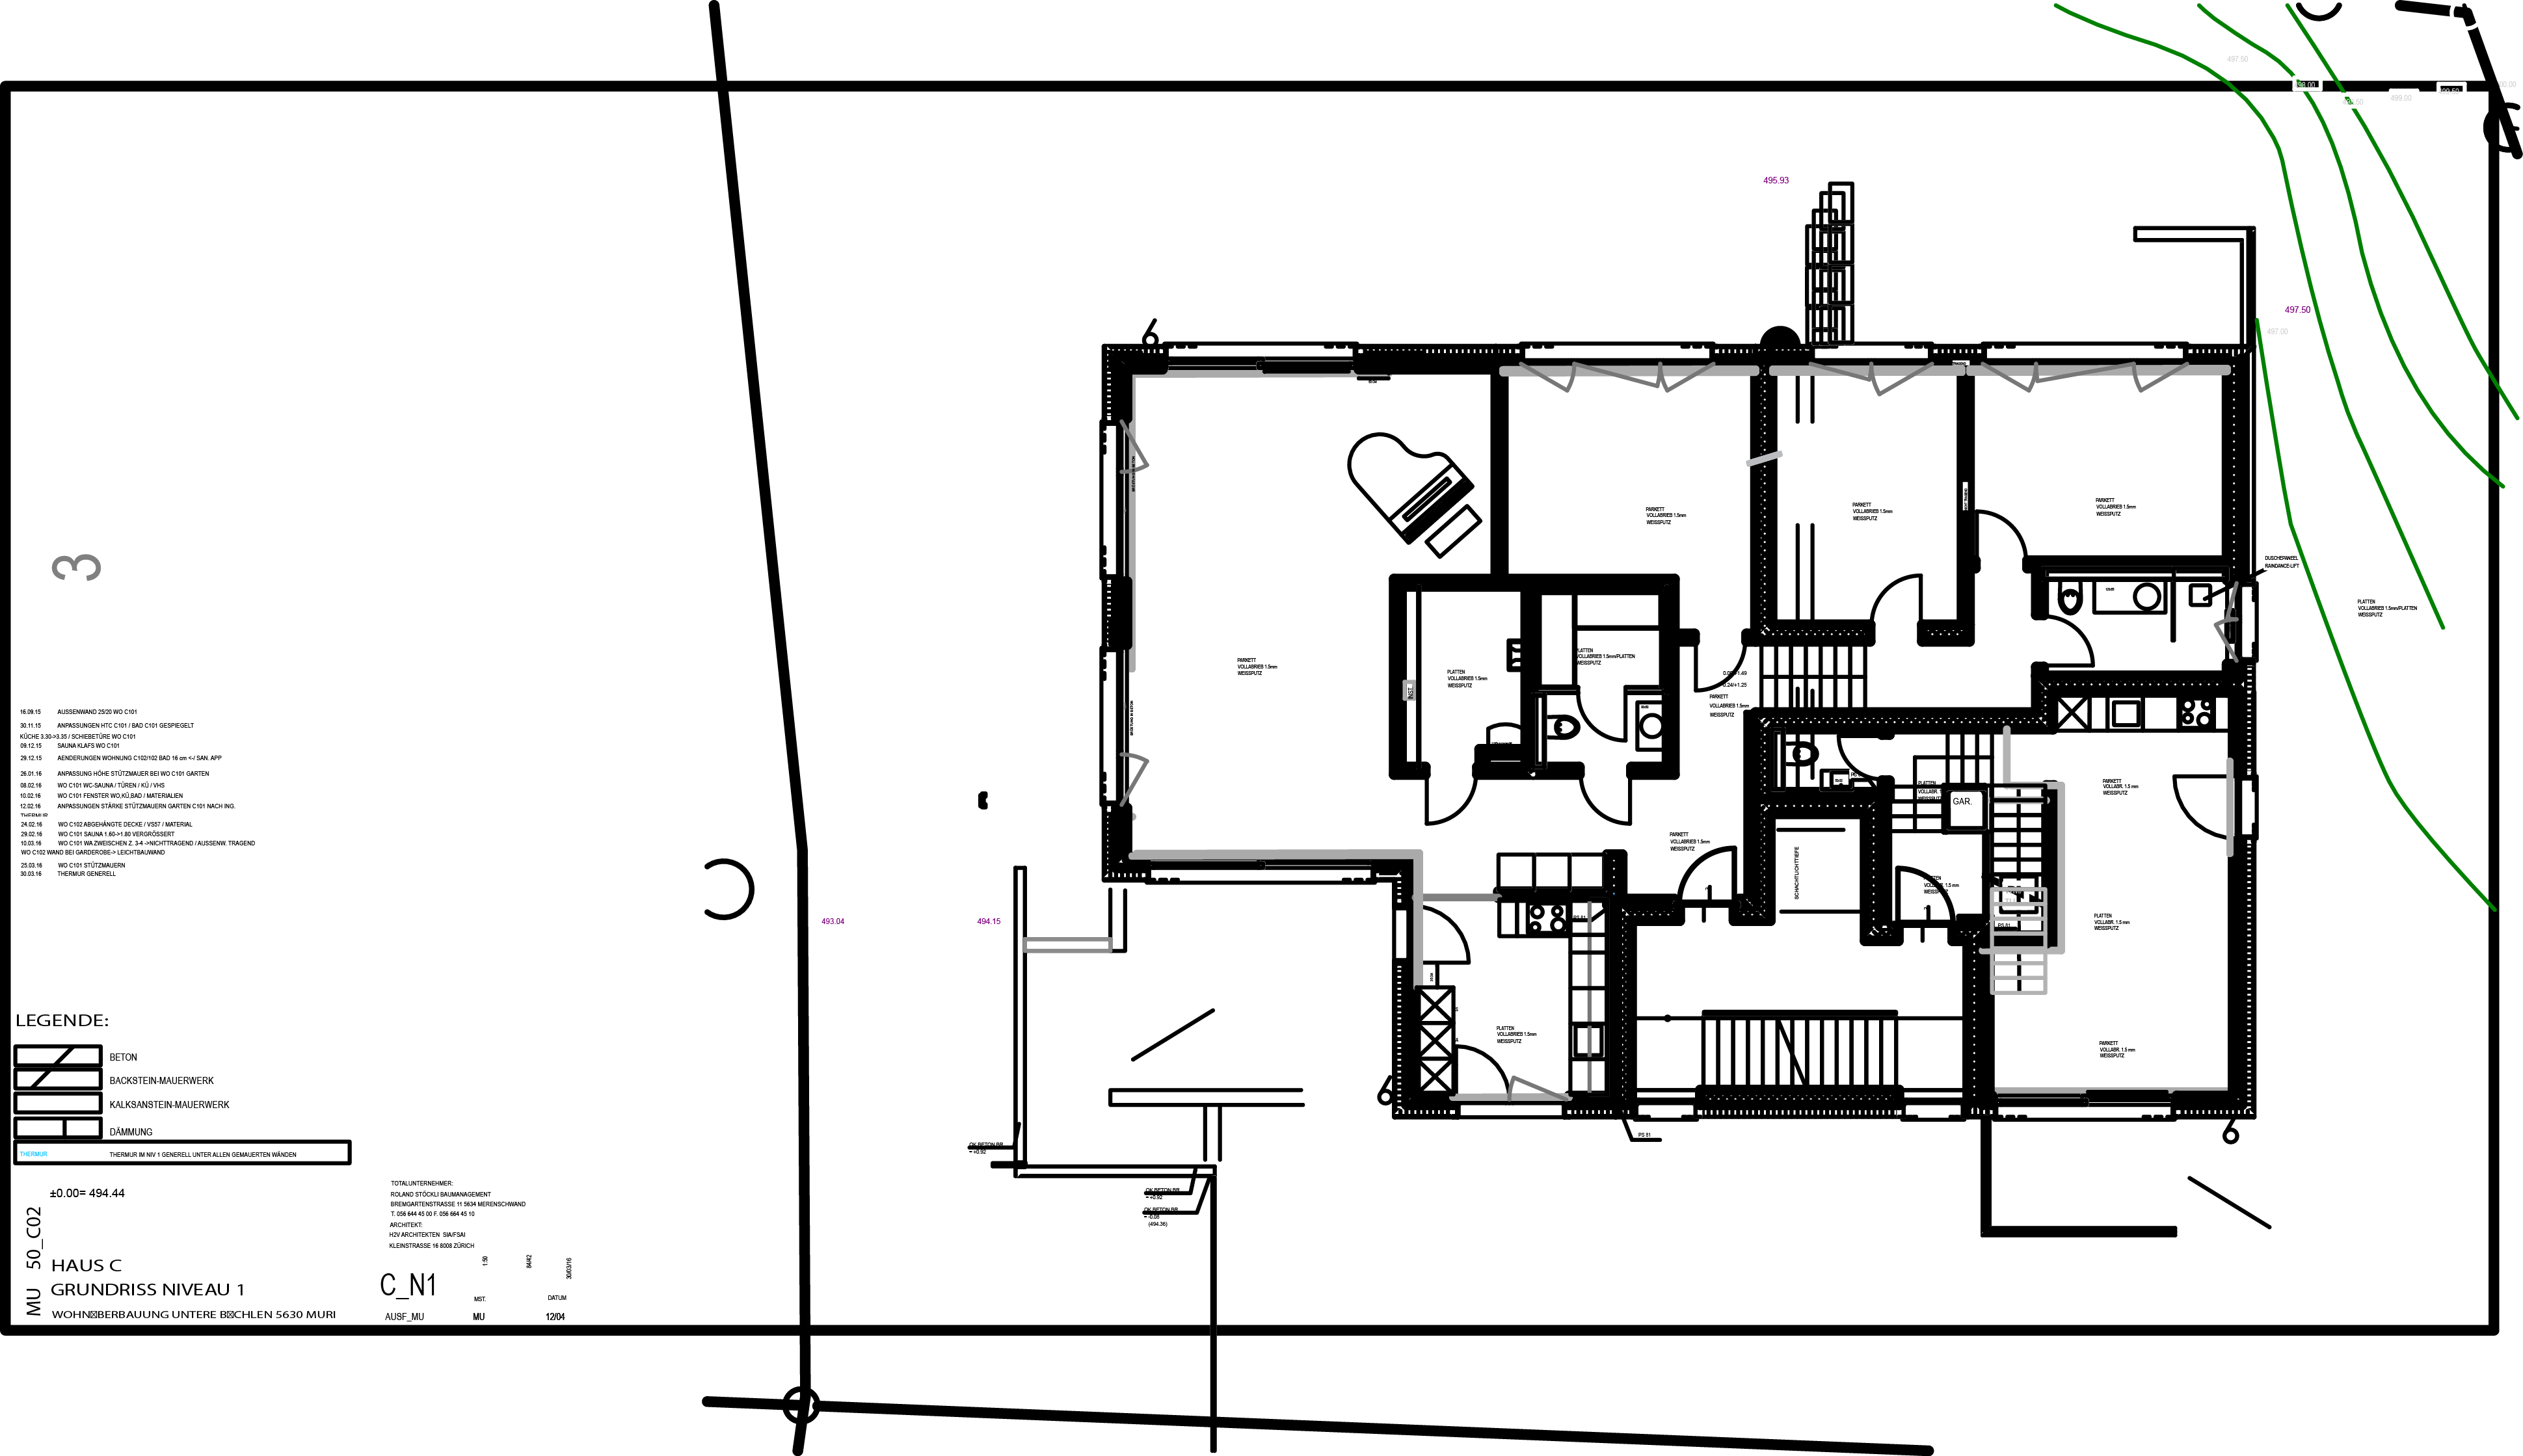
\includegraphics[width=0.5\textwidth]{A_N1.png}\label{fig:A_N1}}
	\hfill
	\subfloat[Image after noise removal.]{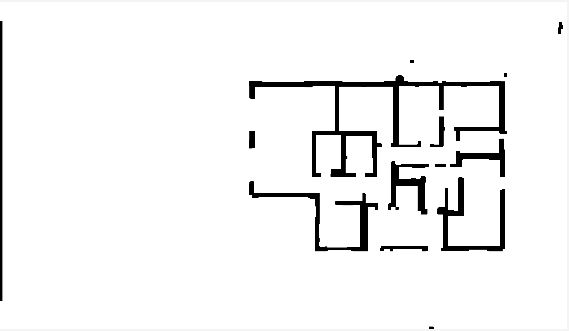
\includegraphics[width=0.4\textwidth]{morphtransuncleaned.jpg}\label{fig:A_N1_Morph}}
	\caption{Before and after of an uncleaned floor plan with noise removal. }
\end{figure}

\begin{figure}[h]
	\centering
	\subfloat[Original image.]{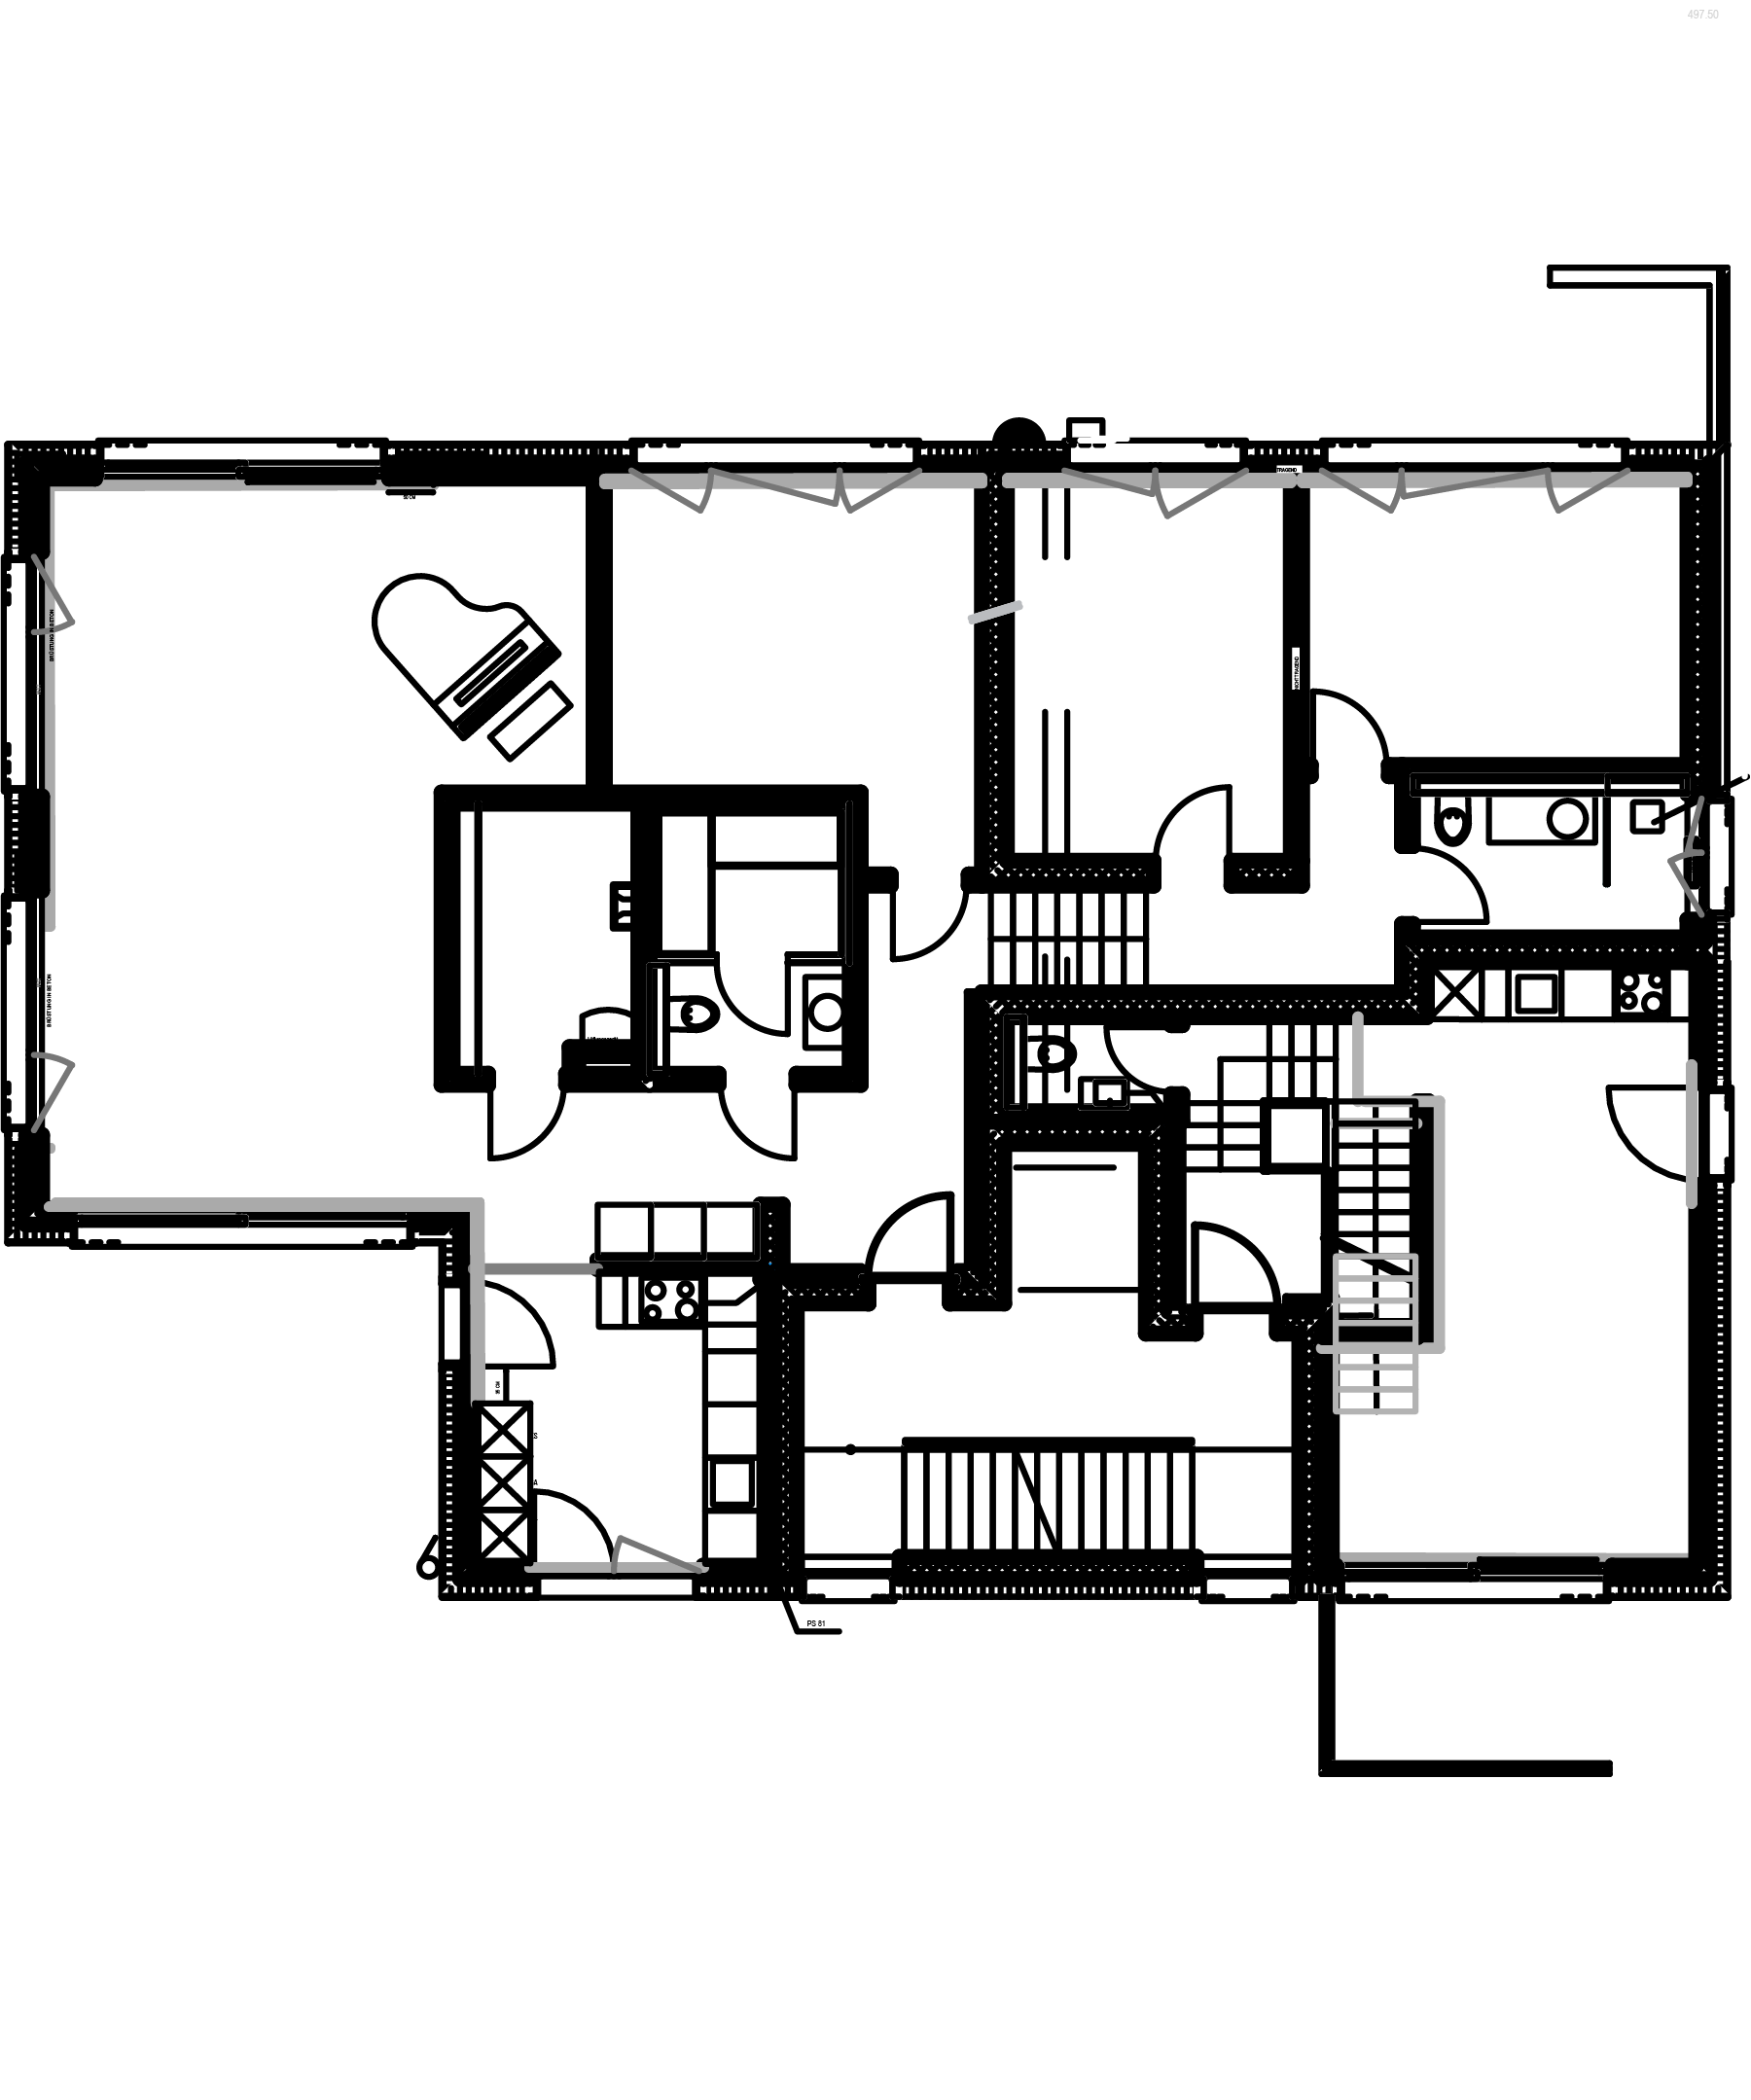
\includegraphics[width=0.5\textwidth]{A_N1_cleaned.png}\label{fig:A_N1_cleaned}}
	\hfill
	\subfloat[Image after noise removal.]{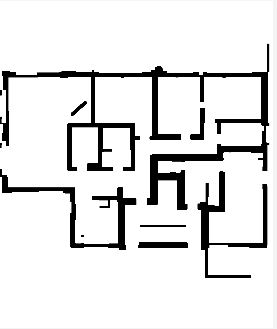
\includegraphics[width=0.4\textwidth]{morphtranscleaned.jpg}\label{fig:A_N1_cleaned_Morph}}
	\caption{Before and after of a cleaned floor plan with noise removal.}
\end{figure}

The figure~\ref{fig:A_N1} is one of the uncleaned testing images before any noise removal. It was cleaned up with an erosion/dilation size of 8. Figure~\ref{fig:A_N1_Morph} is the result of the noise removal. It is easily visible that most of what's left are walls. Due to the thin lines of the windows they get removed in the process. Those will be added later though as they are an important part of the wall to surround the rooms.

The same was done to the cleaned up image. As a result of different image sizes the noise removal was actually worse with the same parameters. This shows that each different image has very specific parameters for an optimal noise removal. This is further discussed in the section \ref{subsec:Parameter Finding}.

As this is not perfect due to the variety of possible objects on a plan, there is the option to delete those beforehand or afterwards with our built in editor. This is so we can manually improve the quality of the outcome of noise removal.

As a result of the noise removal we get an image with very basic information about where the walls are. This will be very important for our next step and other steps to come.
\subsubsection{Normalize Image}
\subsubsection{Distance transformation \& Geodesic dilation}
The distance transformation is used to find the centers of the rooms as explained in section~\ref{subsubsec:Distance transformation}. As its base it needs a cleaned up image of all the walls. It is a result of the noise removal we discussed in the previous section. To find the actual area of the of the room there is further processing with a geodesic dilation needed.

The distance transformation gives us an image that represents the distance from the walls (lines in black) as a gradient of gray values going from dark (close to the wall) to bright (farther away). This means that there will be a center in each room that is very bright and has color values close to white.

\begin{figure}[H]
	\centering
	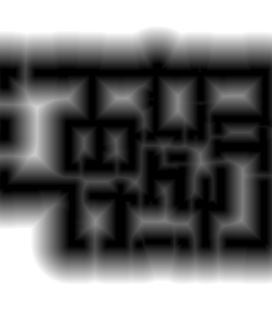
\includegraphics[width=0.8\textwidth]{dist_transform.jpg}
	\caption{Example distance transformation of a architectural floor plan.}
	\label{fig:dist_transform}
\end{figure}

To find the centers there had to be an additional method that provides us with a specific information where these center areas are.
\todo{Discuss specific parameters for each image in parameter finding}
\todo{Distance Transform, Why not Contour Detection}
\subsubsection{Find Center of Distance Transform}  
\subsubsection{Hough transformation}
\subsubsection{JavaCv}
Hough line transformation was the first algorithm we tried using to find the walls in the floor plan. It finds straight lines  
\subsubsection{Harris corner detection}
\subsubsection{Corner sharpening}


\subsubsection{Sparse Point Cloud}
\subsection{Structural Analysis}
test
\todo{Object Detection: TM, Hough Lines, ORB}
\subsubsection{Canny Line Detection} 
\subsubsection{Find Contours}
\subsubsection{Geodesic Dilation}
\subsubsection{Marker Distance Transform}
\subsubsection{HoughP Line Detection}
\subsubsection{Template Matching}
\subsubsection{Gap Closing Alg}
\subsubsection{Simple gap closing}
\subsubsection{Cascade classifier}
The cascade classifier is used for object recognition of doors, windows and other objects that are important for the room detection and zone identification. This algorithm is a machine learning algorithm that has to be trained with positive and negative images. The resulting learned parameters are safed in an XML file. Since this is a crucial part of this project, it is described more detailed than most other algorithms. In the following lines the implementation process is described as well as all the experiences we made during this project.

The basic problem was to find an algorithm that can find objects that vary in their details and regardless of their rotation and size. This is important due to the fact that there is no standard for objects in architectural floor plans that are used by a wide audience of architects. The decision to go with a machine learning approach and not an algorithm that works with heuristics is because we wanted to be able to process a broad variety of floor plans. Regardless wheter they show a small house with just basic features or a big plan with a lot of details and special objects.




\todo{Cascading Classifier: To few samples, Cat images prove, more positive, thickening, polydp, positive negative ratio, more specific negative samples}
\todo{Object Single Cases}
\todo{Gaps Closing: Clustering, Rotation / MinBox}
\subsubsection{Bad results}
\subsubsection{Shape Distance Matching}
\subsubsection{Erosion for better Results}
\subsubsection{Detection with more Pos/Neg}
\subsubsection{Component analysis}
\subsubsection{Border removal}
\subsubsection{Minimum room}
\subsubsection{Exterior wall closing algorithm}
\subsubsection{Polygon approx}
\subsubsection{opening for exterior wall}
\subsubsection{Image size}
As a result of a lot of the testing we found out that images that have too big of a size use a lot of ram to process. Images below 100 kBytes did not affect the heap too much. There was an increased use of RAM due to the program of around 1-2 GB. When images of size 300 kBytes and bigger, the computer used for testing used more than 5 GB of additional RAM to process during one instance. This can lead to huge problems. The program will crash if there is no more RAM available. Therefore it is necessary to reduce the size of the image to a size below 150 kBytes. Otherwise there is no guarantee that the given RAM is enough to process. Especially when there are different programs running. For example an additional architecture program. Those usually use a lot of Heap-Space themselves. \todo{This is wrong, it is dependent on the pixel size not megabytes.}

\subsection{Semantic Analysis}
\subsubsection{NikieRoomDetection}
\subsubsection{Watershed}
The watershed is the core of our room search algorithm. Its purpose is to fill  the unknown areas that are provided in a foreground/background image from previous images. It needs extremely good preprocessing. If it has any previous errors, the resulting rooms will not make sense.

We use the watershed to its ability to find connected rooms with a simple method. It is a simple algorithm that has low computational cost. This and the fact that it was already implemented in openCV makes us use this algorithm.

The algorithm uses a simple image of all the walls as an image to compare to the foreground/background image. This image has been modified with the door recognition algorithm to close all doors within that picture. This is important so rooms are separated when running the watershed algorithm. Additionally we tried to do a window recognition to close the outside walls. As explained in section \todo{Explain why window rec didnt work}, this did not work out as planned. What we instead used was \todo{create alternative to window recognition}. With this method we are able to separate all rooms within a building that has no windows on the inside. Any building that has a courtyard will fail with this method. Our goal was to find a solution that can also deal with this. But due to limited time and no reasonable alternative we chose to go with that.

The background/foreground image is split up in three different zones. The zone with pixel color values of 0 represent the part of the image that are unknown. All pixels with color value \todo{findValue} represent the walls. As for the rooms we chose to mark all center with value \todo{findValue}. The image used for comparison has the same areas with walls as the BG-image. This means that the area for the wall will not expand with the watershed. The only exception is the area where doors or windows were closed. This is based on the assumption that the wall has the same pixel color and the inside of the room has a vastly brighter color.
The bright centers of the room inside the BG-image will expand into the unknown areas close to the walls and fill up the rooms. This will result in an image with several enclosed rooms all having the same pixel color. This will be processed with a modified connected components algorithm to find all the edges or the room.

We ran into several problems during the implementation of this algorithm. The most common problem is that not all doors were found. Additionally not all rooms have doors to separate them. There are also rooms that are separated with just an open space. There are also objects like cabinets that were drawn with thick lines and were identified as a part of the room. This is easily recognizable as a human but can not be differentiated with the algorithms used.

As a solution to the fact that not all the doors are found, there is the option to close doors by hand with the editor. This is the simplest solution that always guarantees success. We also tried to improve door detection with better samples and bigger sample size. This can be found in the section \todo{link section with door detection}.
To erase object from the image we initially planned to do an object detection. There was time to do some additional object detection other than just door and window. Those can be found in the code. But there are too many different object only within those few plans we got to catch them all. To implement all of the and erase those objects is a next step for this project. For now the user has to erase all object that do not get caught by noise removal by hand.
\todo{Watershed}

\subsubsection{Watershed inverse binarization}
\todo{Polygon Smoothing}